% 03-results-and-discussions.tex

% Section Title
\section{RESULTS AND DISCUSSIONS} \label{sec:results}

    \subsection{Baseline Performance: Static vs.\ Dynamic}

        Comparing the static and dynamic scenarios highlights key differences in GNSS signal behavior, measurement stability, and receiver performance. 
        Although both datasets were collected under similar atmospheric conditions, the receiver's motion in the dynamic case introduced visible changes across all GNSS indicators.
    
        \vspace{0.5em}
        \noindent\textbf{Pseudoranges vs Time.} 
        \\The pseudorange measurements reveal distinct trends across scenarios. In Fig. \ref{fig:static_pseudoranges_a} \textbf{more satellites} (e.g., SVs 27, 4, 20, 5, 16, 28, 29, 18) are consistently tracked, exhibiting \textbf{flat trajectories} with minimal variation (range: $\sim$2.1--2.5$\times 10^7$ m). This suggests stable signal acquisition under favorable conditions. In contrast, Fig.\ref{fig:static_pseudoranges_b} displays \textbf{fewer visible satellites} (e.g., SVs 28, 29, 31, 12, 18), with several signals showing abrupt shifts or non-linear behavior (range: $\sim$2.0--2.6$\times 10^7$ m). The reduced satellite count in Plot B implies \textbf{challenging signal reception}, possibly due to environmental interference or motion-induced signal degradation.  


        \begin{figure}[h!]
            \centering
            \begin{subfigure}{0.23\textwidth}
                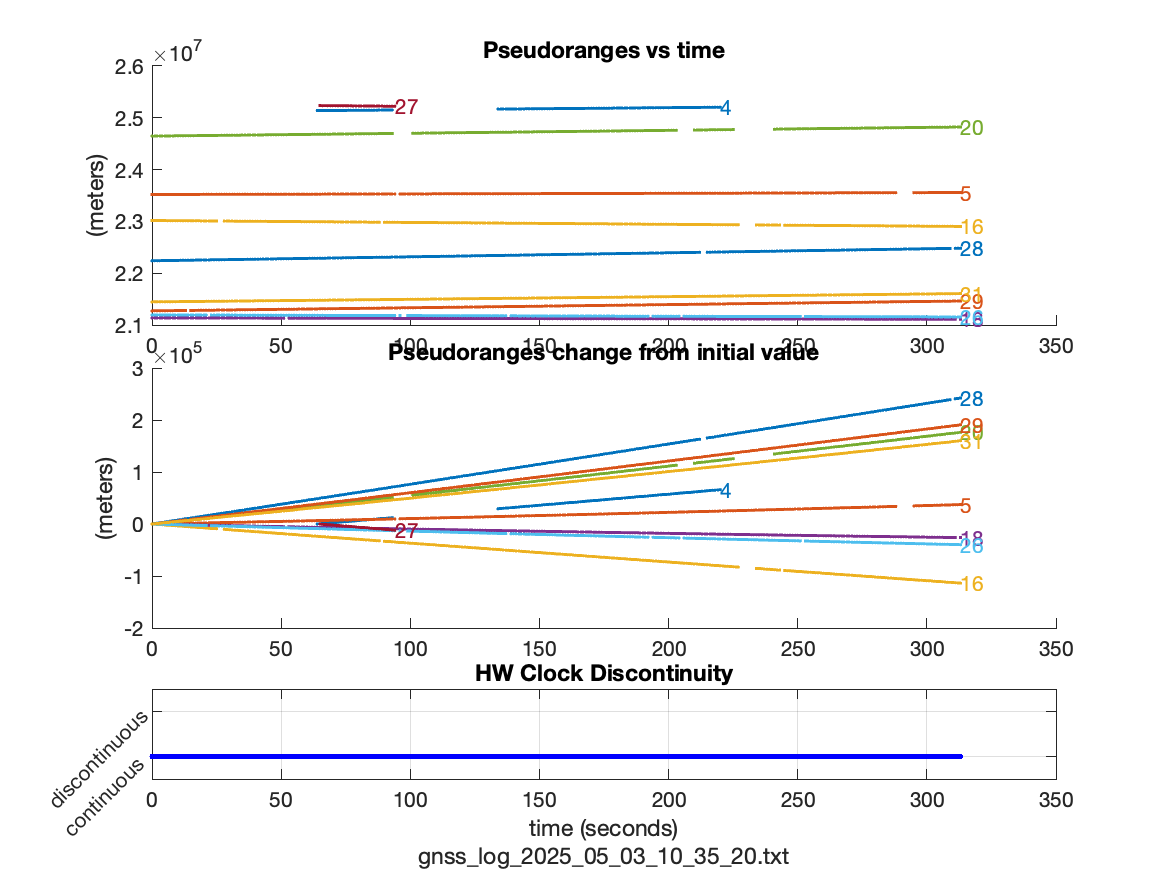
\includegraphics[width=\textwidth]{images/tests/Monte_Cappuccini/png/Samsung_A51_Monte_Cappuccini_fig1.png}
                \caption{Static: Pseudoranges vs time}
                \label{fig:static_pseudoranges_a}
            \end{subfigure}
            \hfill
            \begin{subfigure}{0.23\textwidth}
                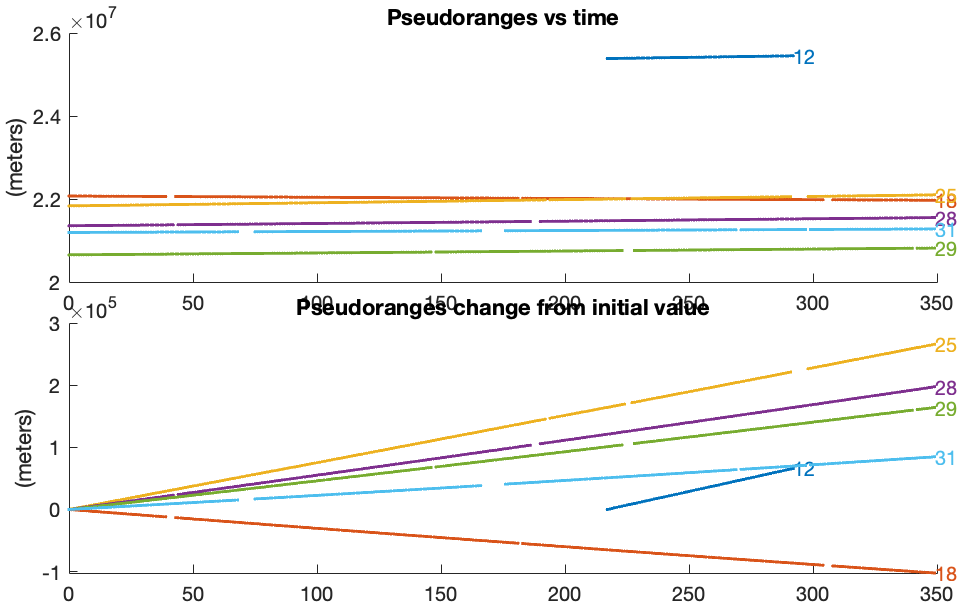
\includegraphics[width=\textwidth]{images/tests/Tram_15_trip_Castello_to_Pescatore/filtered/Samsung_A51_Tram_15_trip_Castello_to_Pescatore_fig1.png}
                \caption{Dynamic: Pseudoranges vs time}
                \label{fig:static_pseudoranges_b}
            \end{subfigure}
        \end{figure}
    

        \vspace{0.5em}
        \noindent\textbf{Pseudorange Change from Initial Value.} 
        \\Deviations from initial values further highlight differences. In Fig. \ref{fig:static_pseudoranges_a}, all tracked satellites follow \textbf{shallow linear trends} ($\pm$0.5--2 m), reflecting predictable signal dynamics. The consistency across satellites (e.g., SVs 27, 28, 29) suggests robust tracking of both strong and weaker signals, including those from higher-elevation satellites. Conversely, Fig. \ref{fig:static_pseudoranges_b} shows \textbf{steeper slopes} (up to $\pm$3 m) and fragmented trends, with notable examples like SV 12 (sudden jump after $\sim$200 s) and SV 18 (continuous negative drift). The variability in Plot B indicates \textbf{intermittent signal loss or multipath effects}, particularly for satellites with marginal signal strength. 

    
        \vspace{0.5em}
        \noindent\textbf{Positioning and Speed.} 
        \\In the  the plots depict positional estimates. Fig. \ref{fig:Position_Speed_a} displays a clustered distribution around its median $(45.059862^\circ, 7.697191^\circ)$, with a $50\%$ confidence ellipse spanning $\sim \pm 15$ m. This indicates stable positioning with minimal drift. In contrast, Fig. \ref{fig:Position_Speed_b} shows a widely scattered pattern centered at $(45.066832^\circ, 7.692336^\circ)$, featuring a $50\%$ ellipse extending $\sim \pm 400$ m. The median in Plot B lacks practical relevance due to extreme positional variability, unlike Plot A’s median, which accurately represents stationary behavior.  

        The middle plots highlight horizontal speed trends. Fig. \ref{fig:Position_Speed_a} exhibits near-zero speeds ($<2$ m/s) with minor oscillations, consistent with negligible movement. Conversely, Fig. \ref{fig:Position_Speed_b} reveals erratic fluctuations, including a peak exceeding $20$ m/s.

        The bottom plots compare HDOP and satellite visibility. Fig. \ref{fig:Position_Speed_a} maintains low HDOP ($<5$) with consistent visibility of 8–10 satellites, reflecting robust signal geometry. In contrast, Fig. \ref{fig:Position_Speed_b} shows elevated HDOP (up to $\sim 10$) alongside reduced satellite counts (4–6), indicating degraded tracking conditions.

        \begin{figure}[h!]
            \centering
            \begin{subfigure}{0.23\textwidth}
                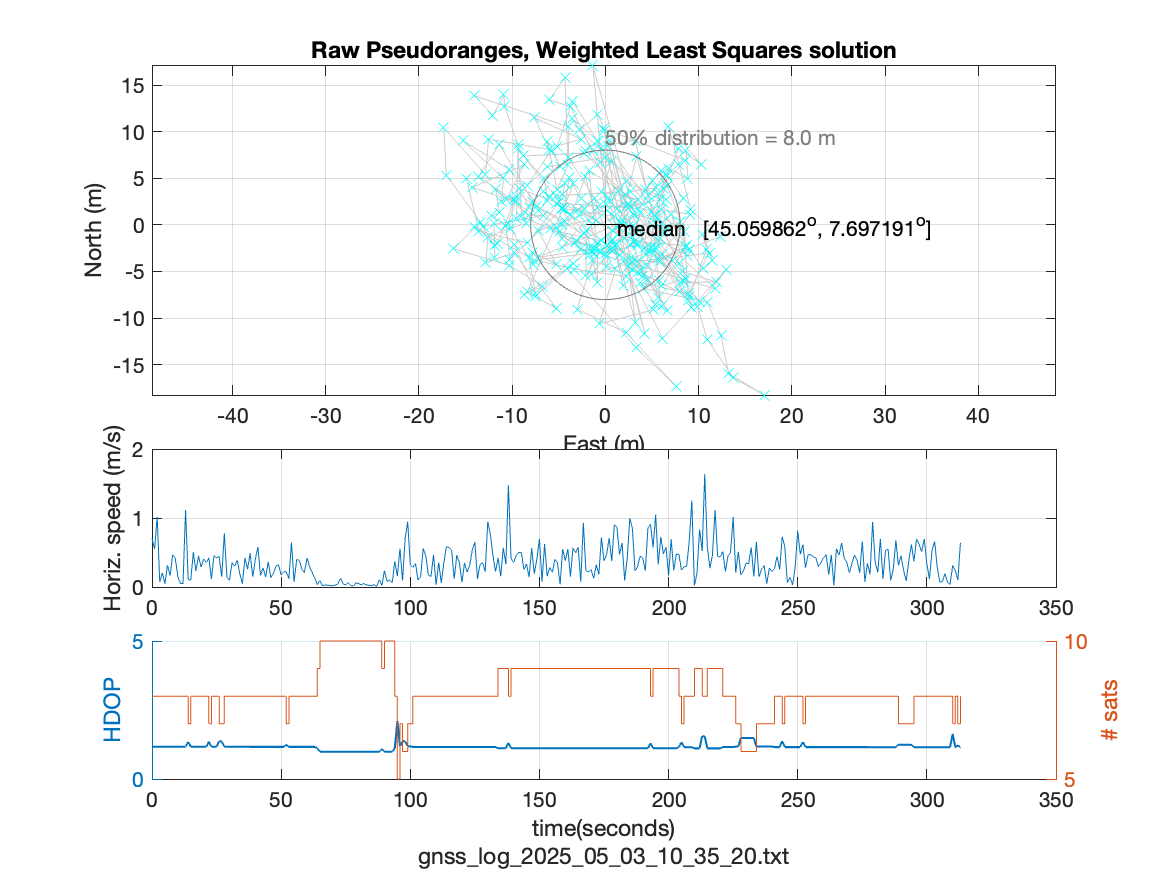
\includegraphics[width=\textwidth]{images/tests/Monte_Cappuccini/png/Samsung_A51_Monte_Cappuccini_fig4.png}
                \caption{Static: Position, Speed, HDOP}
                \label{fig:Position_Speed_a}
            \end{subfigure}
            \hfill
            \begin{subfigure}{0.23\textwidth}
                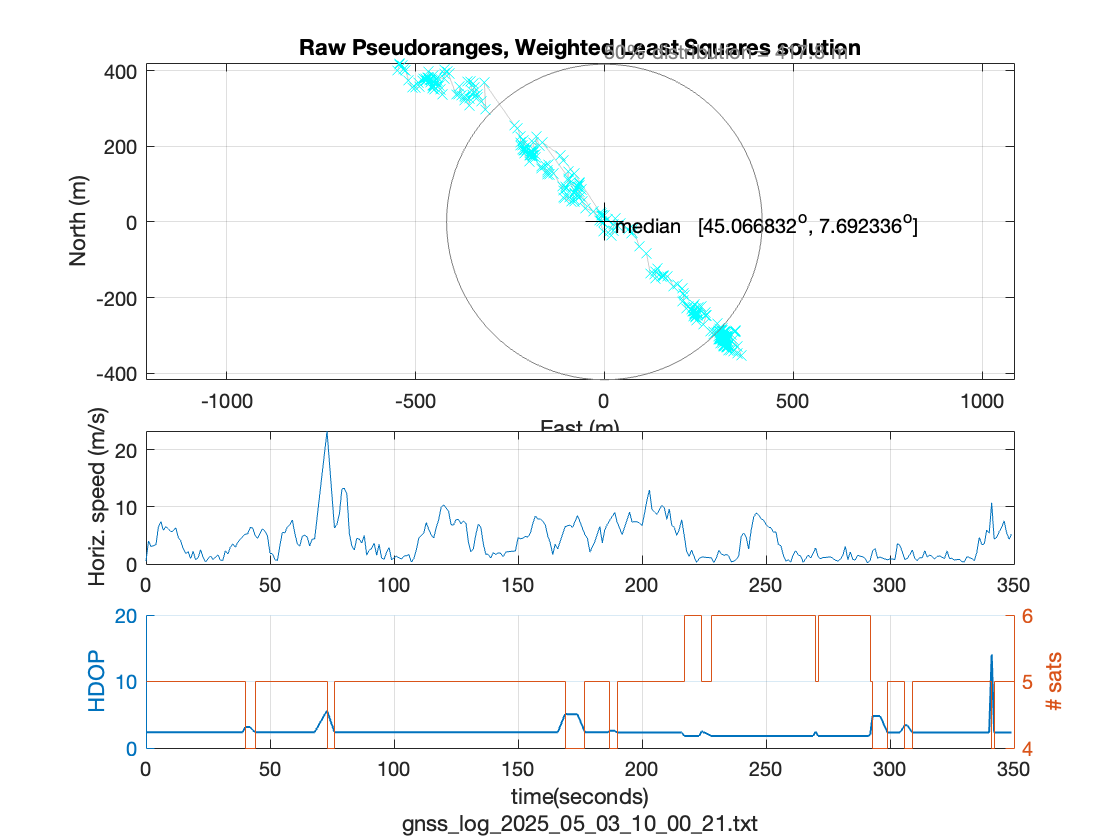
\includegraphics[width=\textwidth]{images/tests/Tram_15_trip_Castello_to_Pescatore/filtered/Samsung_A51_Tram_15_trip_Castello_to_Pescatore_fig4.png}
                \caption{Dynamic: Position, Speed, HDOP}
                \label{fig:Position_Speed_b}
            \end{subfigure}
        \end{figure}
    
        \vspace{0.5em}
        \noindent\textbf{State Offsets and Timing Bias.} 
        \\The \textbf{top plots} illustrate position state offsets relative to the median. In Fig. \ref{fig:WLS_a}, deviations in latitude, longitude, and altitude remain tightly constrained within $\sim \pm 50$ m, with smooth, gradual fluctuations indicating stable signal tracking. In contrast, Fig. \ref{fig:WLS_b} exhibits extreme offsets exceeding $\pm 500$ m, punctuated by abrupt spikes (e.g., a $\sim 600$ m jump near 150 seconds).  

        The \textbf{second plot} shows clock bias (common bias) trends. Both plots exhibit linear growth, but in Fig. \ref{fig:WLS_a} increases steadily ($\sim 200$ ns over 350 seconds), reflecting predictable receiver clock drift. Fig. \ref{fig:WLS_b} escalates more sharply ($\sim 250$ ns over the same interval), with a notable dip aligning with the positional spike in the top plot. This correlation implies transient disruptions affecting both position and timing stability in Plot B.  

        Velocity state estimates (\textbf{third plot}) further differentiate the two scenarios. Fig. \ref{fig:WLS_a} shows near-zero velocities (all components $\leq 2$ m/s), consistent with negligible movement. Fig. \ref{fig:WLS_b}, however, displays pronounced oscillations, particularly in the northward direction (peaks $\sim \pm 20$ m/s), indicating rapid or inconsistent motion.  

        The \textbf{bottom plots} depict common frequency offset trends. Fig. \ref{fig:WLS_a} maintains a stable trajectory near $0.8$ ppm, with minor perturbations. Fig. \ref{fig:WLS_b} shows greater variability, including a sharp downward deviation during the positional spike. This suggests that signal degradation or motion-induced errors propagate to both position and frequency estimates in Plot B, unlike the consistent behavior seen in Plot A.  

        \begin{figure}[h!]
            \centering
            \begin{subfigure}{0.23\textwidth}
                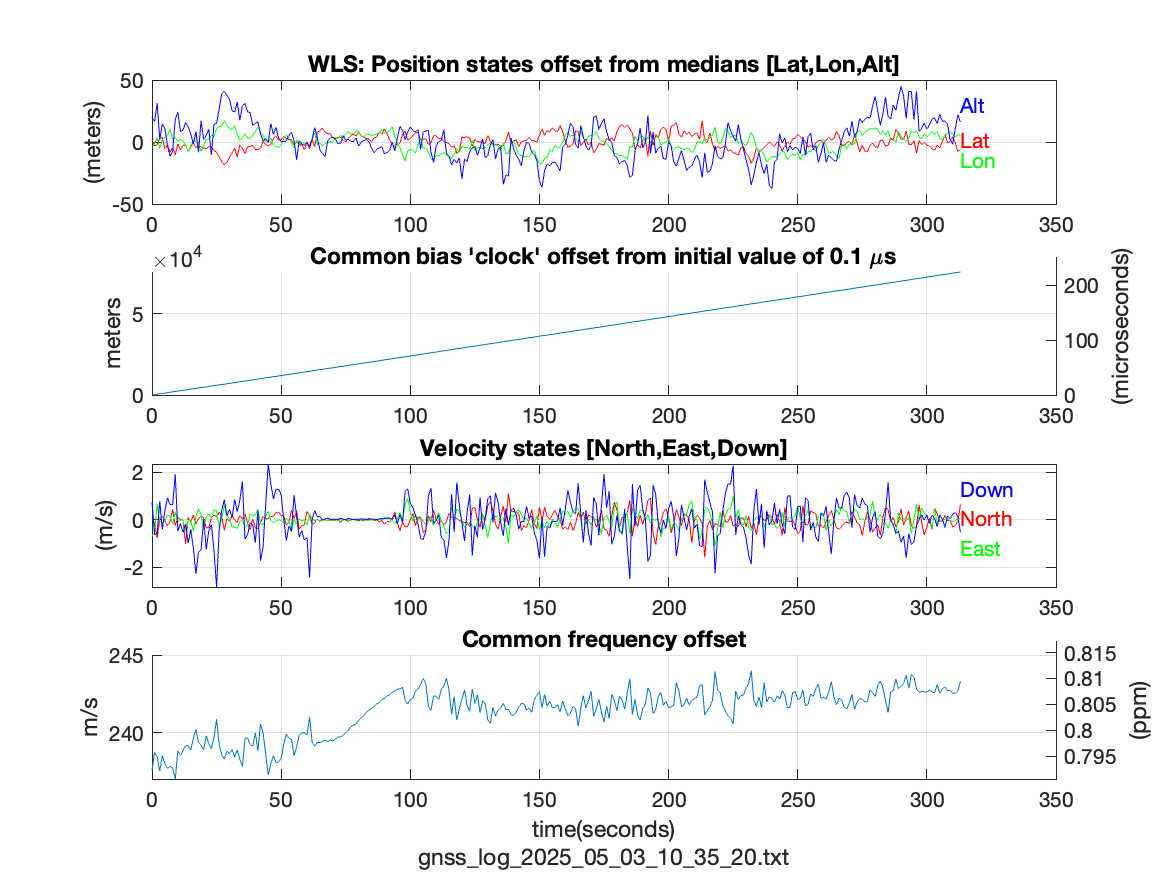
\includegraphics[width=\textwidth]{images/tests/Monte_Cappuccini/png/Samsung_A51_Monte_Cappuccini_fig5.png}
                \caption{Static: WLS states and bias}
                \label{fig:WLS_a}
            \end{subfigure}
            \hfill
            \begin{subfigure}{0.23\textwidth}
                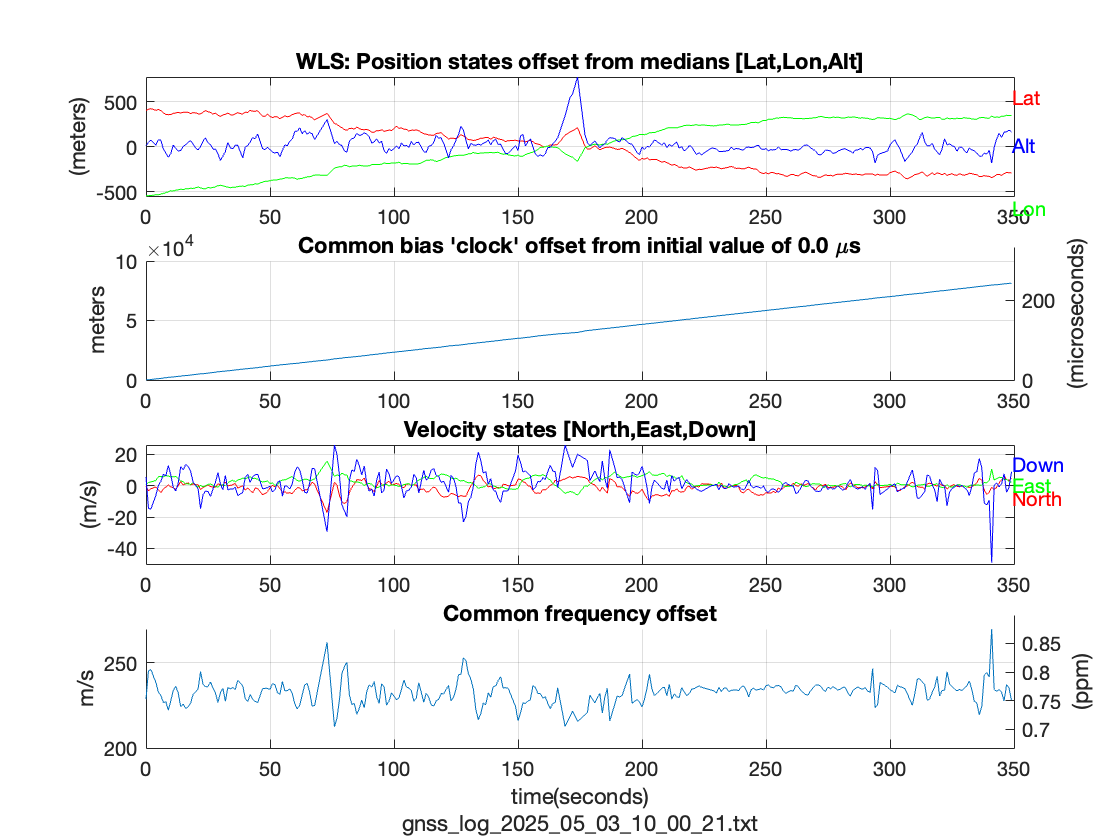
\includegraphics[width=\textwidth]{images/tests/Tram_15_trip_Castello_to_Pescatore/filtered/Samsung_A51_Tram_15_trip_Castello_to_Pescatore_fig5.png}
                \caption{Dynamic: WLS states and bias}
                \label{fig:WLS_b}
            \end{subfigure}
        \end{figure}
    
    \medskip
    \noindent
    These measurements highlight the importance of scenario-aware processing: identical hardware,
    firmware, and atmospheric conditions can yield centimetre-per-second stability on a quiet
    terrace, yet the very same setup will produce hundred-metre excursions once placed on a moving
    tram through an urban canyon.

    \subsection{Impact of Spoofed Position}

        In a spoofing attack, counterfeit signals are broadcast to mimic GNSS transmissions, often altering their timing, amplitude, or content. 
        Typically, these deceptive signals are sent at higher power than the originals to mislead navigation systems. 
        In our experiment, however, spoofing was implemented purely in software by adjusting the perceived reception time inside the professor’s script to simulate spoofing behavior.
            
        \noindent For the spoofed test we manually injected the coordinates of \textbf{Piazza Vittorio Veneto} (45.064749, 7.695466) — a location adjacent to our true survey point — directly into the processing script. 
        As shown in the plots, this causes the solver to converge exactly at the Piazza Vittorio Veneto coordinates rather than the true measurement site, introducing a horizontal displacement of several hundred metres.
        
        \noindent Despite this spatial shift, all raw observables remain essentially unchanged relative to the normal run:
        
        \begin{itemize}
            \item \textbf{Carrier-to-noise density (C/N):} Histograms and time-series trace exactly overlap those of the baseline, confirming no change in received signal strength.
            \item \textbf{Dilution of precision (PDOP):} The satellite geometry quality curve is identical, indicating unchanged constellation geometry.
            \item \textbf{Pseudorange residuals:} The overall spread remains the same, but the entire residual distribution is offset by the constant delay corresponding to the spoofed displacement.
        \end{itemize}



        \begin{figure}[h!]
            \centering
            \begin{subfigure}{0.23\textwidth}
                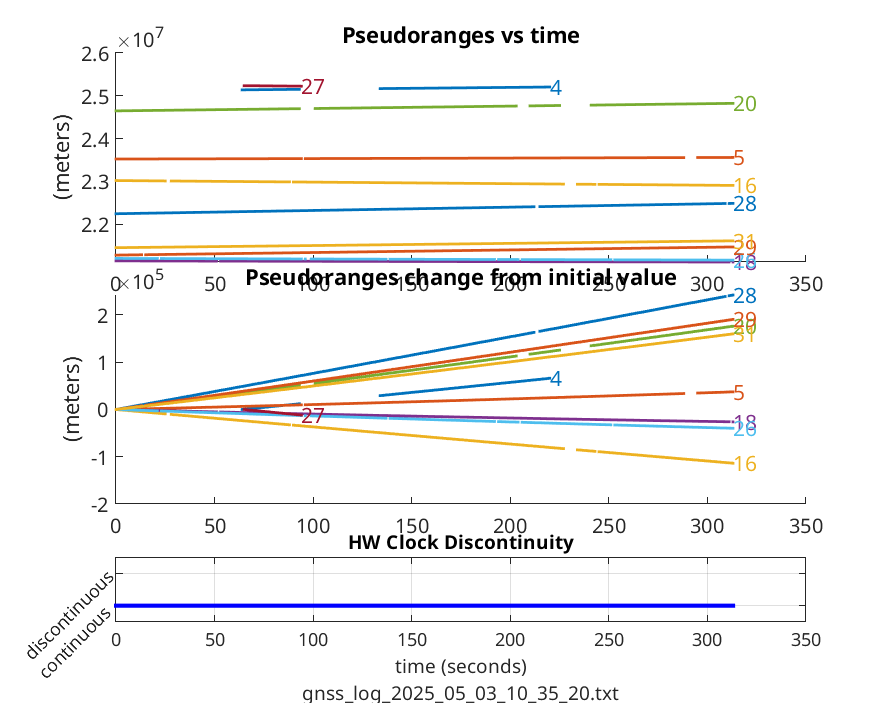
\includegraphics[width=\textwidth]{images/tests/Monte_Cappuccini/Spoofing/task5_figures/Samsung_A51_Monte_Cappuccini_fig1.png}
                \caption{Spoofed: Pseudoranges vs time}
            \end{subfigure}
            \hfill
            \begin{subfigure}{0.23\textwidth}
                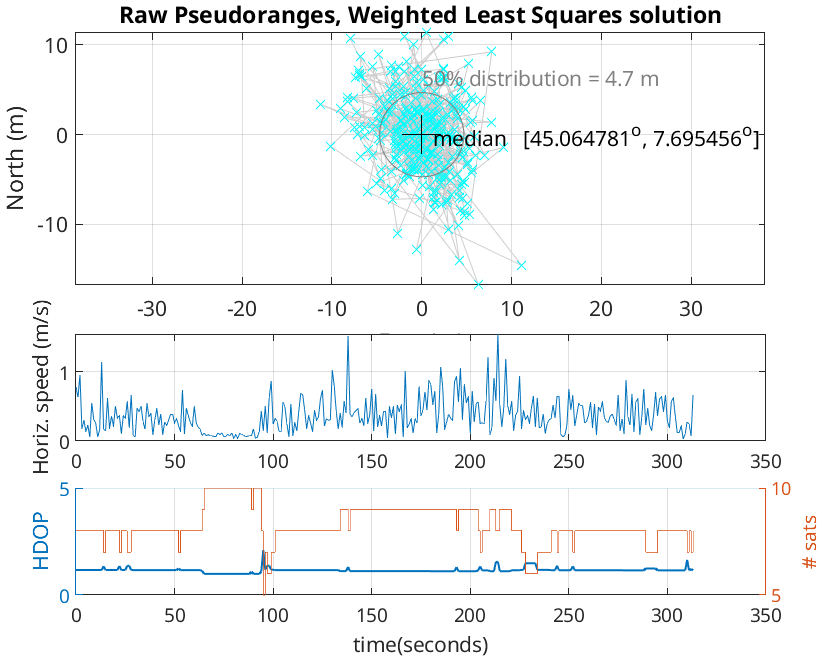
\includegraphics[width=\textwidth]{images/tests/Monte_Cappuccini/Spoofing/task5_figures/Samsung_A51_Monte_Cappuccini_fig4.png}
                \caption{Spoofed: Position, Speed, HDOP}
            \end{subfigure}
        \end{figure}


        \begin{figure}[h!]
            \centering
            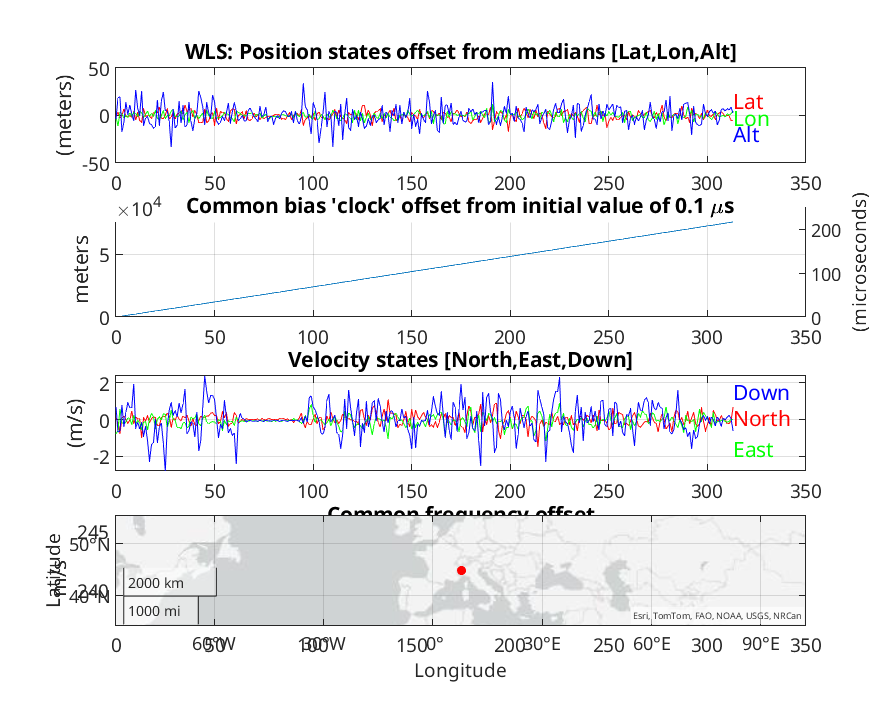
\includegraphics[width=0.9\columnwidth]{images/tests/Monte_Cappuccini/Spoofing/task5_figures/Samsung_A51_Monte_Cappuccini_fig5.png}
            \caption{Spoofed: WLS states and bias}
        \end{figure}

        
        \noindent Additionally, the 50\% (interquartile) range in the median-error distribution shrinks from approximately 8 m in the genuine case to about 4.7 m under spoofing. 
        This reduction occurs because the solver consistently “locks” onto the spoofed coordinate, decreasing variability around that false point.

    \subsection{Effects of Timing Delays}

        In this delayed-spoofing scenario we again target the same true survey point but now introduce a software-only replay delay: the spoofer “listens” to genuine signals, waits 1 ms, then injects the spoofed Piazza Vittorio Veneto coordinates starting at 50 s into the run. 
        The key parameters are set as:

        \begin{verbatim}
cfg.delay   = 1e-3;
cfg.t_start = 50;
        \end{verbatim}


        \begin{figure}[h!]
            \centering
            \begin{subfigure}{0.23\textwidth}
                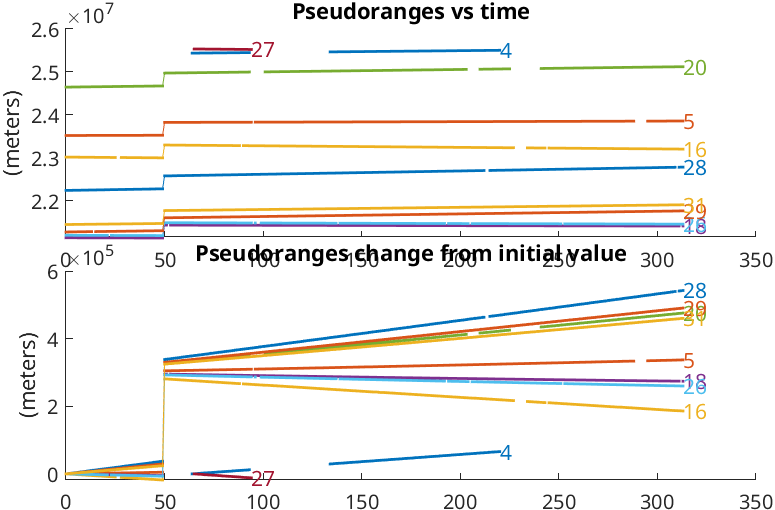
\includegraphics[width=\textwidth]{images/tests/Monte_Cappuccini/Spoofing/task6_figures/Samsung_A51_Monte_Cappuccini_fig1.png}
                \caption{Delay: Pseudoranges vs time}
            \end{subfigure}
            \hfill
            \begin{subfigure}{0.23\textwidth}
                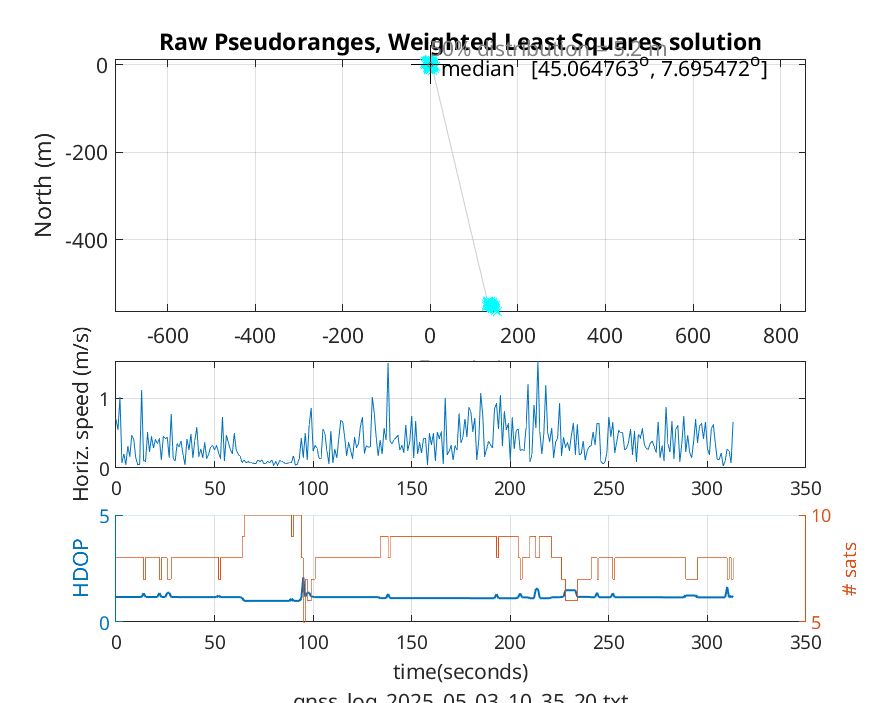
\includegraphics[width=\textwidth]{images/tests/Monte_Cappuccini/Spoofing/task6_figures/Samsung_A51_Monte_Cappuccini_fig4.png}
                \caption{Delay: Position, Speed, HDOP}
            \end{subfigure}
        \end{figure}

                \begin{figure}[h!]
            \centering
            \begin{subfigure}{0.23\textwidth}
                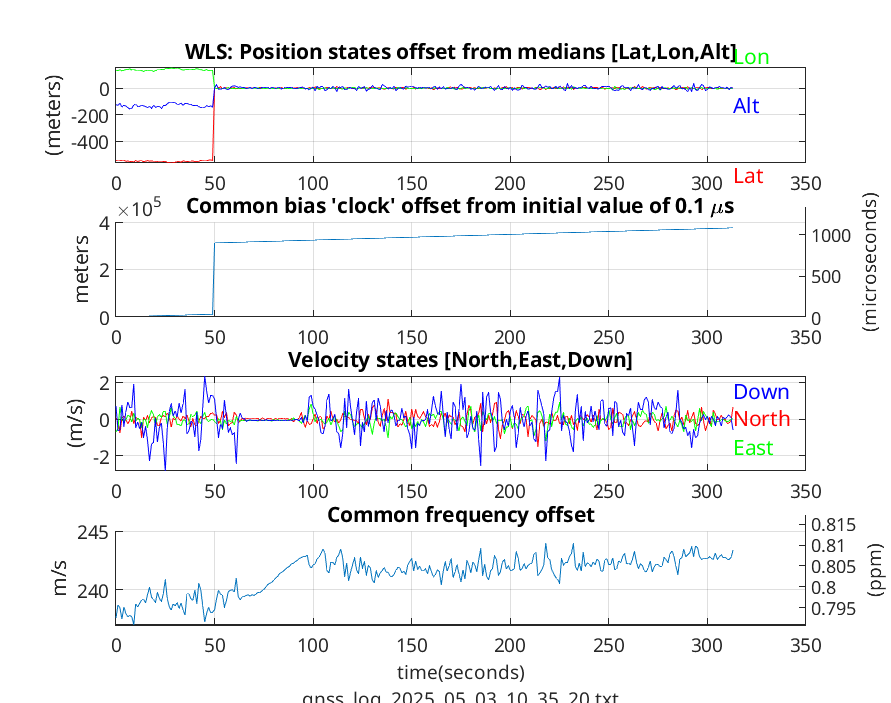
\includegraphics[width=\textwidth]{images/tests/Monte_Cappuccini/Spoofing/task6_figures/Samsung_A51_Monte_Cappuccini_fig5.png}
                \caption{Delay: WLS states and bias}
            \end{subfigure}
            \hfill
            \begin{subfigure}{0.23\textwidth}
                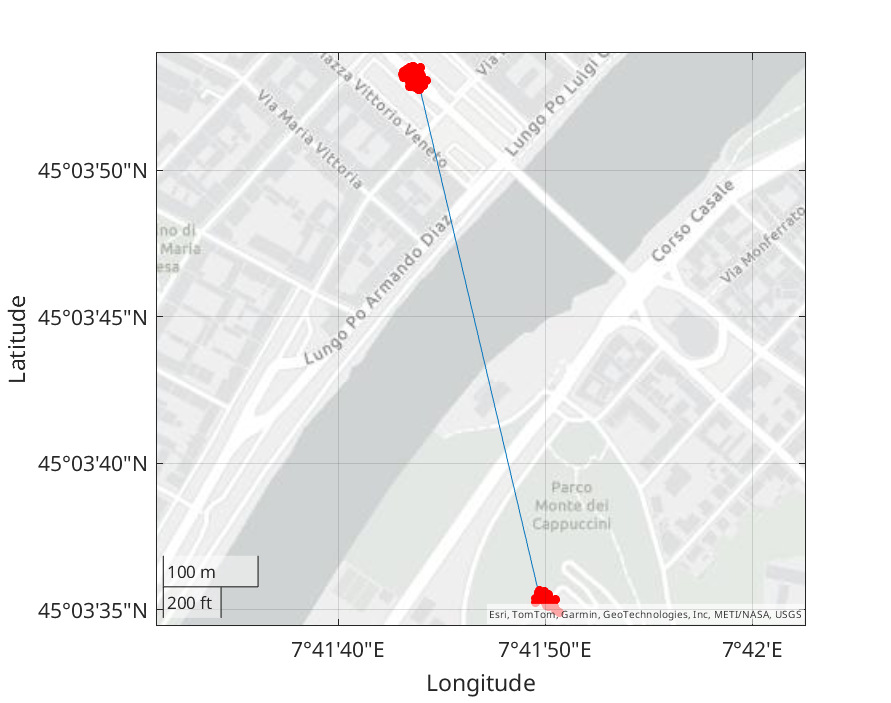
\includegraphics[width=\textwidth]{images/tests/Monte_Cappuccini/Spoofing/task6_figures/Samsung_A51_Monte_Cappuccini_fig6.png}
                \caption{Delay: Position}
            \end{subfigure}
        \end{figure}

        \noindent As visible in the plots, all observables remain nominal until t=50 s, at which point the solver's estimated position and receiver clock-bias exhibit a clear discontinuity as the spoof takes effect.

        \begin{itemize}
            \item \textbf{Position solution:} Prior to 50 s, the estimated coordinate coincides with the true static point. Immediately after 50 s, the solution jumps to the spoofed Piazza Vittorio Veneto location, replicating the static-spoof offset of several hundred metres.  
            \item \textbf{Receiver clock-bias:} A sudden step of appears in the estimated receiver clock-bias track, directly corresponding to the 1 ms replay delay needed to shift the range solution by the planar offset.  
            \item \textbf{Carrier-to-noise density (C/N):} The C/N time-series shows no amplitude change at t=50 s—signal strength is unaffected by delay.  
            \item \textbf{Dilution of precision (PDOP):} Satellite geometry quality remains continuous and invariant through the spoof onset.  
            \item \textbf{Pseudorange residuals:} Residuals maintain the same spread, but their mean shifts abruptly at 50 s by the additional delay delta t.  
        \end{itemize}
        
        \noindent From a solver-stability perspective, the sudden time bias causes an immediate step in both position and clock-bias, sometimes triggering a brief convergence glitch (extra iterations or loss of fix) as the estimator re-optimizes. 
        Even a 1 ms replay delay can therefore introduce a large positional error and matching clock-bias shift without altering any standard observables. Detecting such covert delay-based spoofing thus requires monitoring for timing discontinuities.

    \subsection{Interference Effects}
    
        % If performed, explain signal degradations, cycle slips, and accuracy loss

        % content
